% !TEX root = ../report.tex
\section{Die Datencontainer}
\begin{Spacing}{\mylinespace}

Um die Echtzeitfähigkeit unseres Systems wieder herzustellen, benötigt es der GPU-Unterstützung.
Bevor wir in technische Details verfallen, werden wir einen kleinen Exkurs machen wie GPUs eigentlich arbeiten.

\subsection{Die GPU}
CPUs und GPUs weisen grundlegend verschiedene Architekturen auf. 

\begin{figure}[h!]
	\vspace*{30px}
	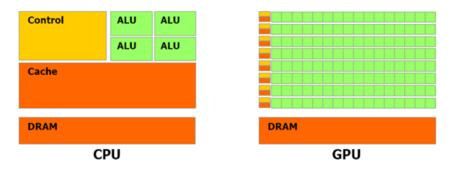
\includegraphics[width=\columnwidth]{graphics/GPUvsCPU.jpg}	
	\caption{GPU-Architektur}
	\label{fig:GPUvsCPU}
\end{figure}
TODO: geklaut hier: http://www.tomshardware.de/CUDA-Nvidia-CPU-GPU,testberichte-240065-2.html

Während eine CPU einen relativ großen Befehlssatz hat um Ganz- oder Fließkommazahlen zu verarbeiten, besitzt hingegen eine GPU einen sehr kleinen Befehlsatz und kann lediglich Fließkommazahlen verarbeiten.
Der große Vorteil einer GPU jedoch ist das sie die Möglichkeit besitzt Berechnungsaufgaben an verschiedene kleinere CO-Prozessoren sogenannte Shader-Units abzugeben.
Durch das zuweisen einer Aufgabe pro Shader-Unit erlaubt eine GPU somit das hoch-parallele abarbeiten von Aufgaben - solange diese unabhängig voneinander sind.
Diese parallele Programmierung hat jedoch auch Nachteile.
Nicht nur das es einer speziellen Programmierung benötigt - sogenannte Shader-Programmierung (Shader-Programme).
Sondern es setzt auch Vorraus, das jede Shader-Unit das gleiche Shader-Programm ausführt.
Besitzen jedoch die zu verarbeitenden Berechnungen genug Unabhänigkeit, so kann eine erhebliche Beschleunigung durch den Einsatz einer GPU welche meist hunderte von Shader-Units besitzt erzielt werden.


\subsection{GPU-Programmierung}
GPUs und CPUs besitzen unabhängigen Speicher es benötigt somit nicht nur spezieller Programme, sondern auch den schwierigen Teil der GPU Programmierung - den Datentransport zwischen den Speichern.
Zur Vereinfachung nehmen wir in nachfolgenden Kapiteln an, das wir folgendes Viereck zeichnen möchten.

\begin{figure}[h!]
	\vspace*{100px}
	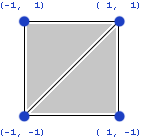
\includegraphics[height=30px]{graphics/quad.png}	
	\caption{Das Viereck}
	\label{fig:Viereck}
\end{figure}

\subsubsection{Indexbuffer}

\subsubsection{GPU-Programmierung}

\subsection{Datencontainer}
\end{Spacing}
\clearpage
%% End Of Doc